\chapter{Räumliches Lernen auf Graphen}
\label{raeumliches_lernen}

Das \emph{räumliche Lernen auf Graphen} basiert auf der direkten Überführung der Definition einer Faltung auf zweidimensionalen Bildern \bzw{} regulären Gittern über ein räumlich verschiebbares Fenster.
Ähnlich wie die Faltung in \glspl{CNN} wird dafür über eine Anordnung der Knoten mit festgelegter Schrittweite iteriert und für diese jeweils eine feste Menge an Nachbarsknoten bestimmt, die das Fenster \bzw{} das Receptive-Field eines jeden Knotens beschreiben~\cite{patchy}.
Aufgrund der gleichmäßigen räumlichen Anordnung der Pixel \bzw{} Knoten auf einem regulären Gitter ist die Definition einer Abtastfolge der Knoten und einer jeweiligen Nachbarschaftsbestimmung mit fester Größe und Ordnung recht trivial, wohingegen solche Definitionen im Kontext von willkürlichen Graphen aufgrund ihrer \ggf{} fehlenden räumlichen (oder zeitlichen) Anordnung nicht gleich ersichtlich erscheinen.

\citeauthor{patchy} definieren in ihrer Arbeit~\cite{patchy} einen solchen räumlichen Faltungsoperator auf Graphen, der im Folgenden vorgestellt und anschließend in den Kontext von Graphen im zweidimensionalen euklidischen Raum überführt wird.

\section{Spektrale Graphentheorie}
\label{spektrale_graphentheorie}

Es gibt 2 große Quellen hier:
\begin{itemize}
  \item Spectral Graph Theory by Chung
  \item Discrete Laplace-Beltrami Operator
\end{itemize}
+ 5 zum Lernen:
\begin{itemize}
  \item Semi Supervised Classification
  \item Fast Localized Spectral Filterung
  \item Wavelets on Graphs via Spectral Graph Theory
  \item The Emerging Field of Signal Processing on Graphs
  \item How powerful are Graph Convolutions? (Review)
\end{itemize}

\subsection{Eigenwerte und Eigenvektoren reell symmetrischer Matrizen}
\label{eigenwerte_symmetrischer_matrizen}

\todo{intro}

$\ma{M} \in \gls{R}^{N \times N}$.
$\gls{eiv} \in \gls{R}^{N}$, $\gls{eiv} \neq \mathbf{0}$.
$\gls{lambda} \in \gls{R}$.
\emph{Eigenwertproblem} $\ma{M}\gls{eiv} = \gls{lambda}\gls{eiv}$.
Zu einem \emph{Eigenwert} $\gls{lambda}$ gibt es unendlich viele (skalierte) \emph{Eigenvektoren} \gls{eiv}.
Wir definieren den Eigenvektor \gls{eiv} eines Eigenwertes \gls{lambda} daher eindeutig über die Bedingung $\left\|\gls{eiv}\right\|_2 = 1$.
Sei \ma{M} weiterhin symmetrisch, \dhe{} $\ma{M} = \ma{M}^{\top}$.
Dann gilt für zwei unterschiedliche Eigenvektoren $\gls{eiv}_1$ und $\gls{eiv}_2$, dass $\gls{eiv}_1 \gls{ortho} \gls{eiv}_2$.
Weiterhin hat \ma{M} genau $N$ reelle Eigenwerte mit ${\left\{\gls{lambda}_i\right\}}_{i=1}^N$.

Wir definieren zu \ma{M} die orthogonale \emph{Eigenvektormatrix} $\gls{Eiv} \coloneqq \left[\gls{eiv}_1, \ldots, \gls{eiv}_n\right] \in \gls{R}^{N \times N}$, wobei $\gls{Eiv}\gls{Eiv}^{\top}=\gls{I}$, und dessen korrespondierende Eigenwertdiagonalmatrix $\gls{Lambda} \coloneqq \gls{diag}\left({\left[\gls{lambda}_1, \ldots, \gls{lambda}_N\right]}^{\top}\right)$, \dhe{} $\gls{Lambda}_{ii} = \gls{lambda}_i$.
Dann gilt $\ma{M}\gls{Eiv} = \gls{Eiv}\gls{Lambda}$ und insbesondere ist \ma{M} diagonalisierbar über
\begin{equation*}
  \ma{M} = \ma{M}\gls{Eiv}\gls{Eiv}^{\top} = \gls{Eiv}\gls{Lambda}\gls{Eiv}^{\top}.
\end{equation*}

Weiterhin gilt für die $k$te Potenz von $\ma{M}$, $k \in \gls{N}$,
\begin{equation}
  \ma{M}^k = {\left(\gls{Eiv}\gls{Lambda}\gls{Eiv}^{\top}\right)}^k = \gls{Eiv}\gls{Lambda}^k\gls{Eiv}^{\top}.
  \label{eq:matrix_potenz}
\end{equation}

Dieser Zusammenhang lässt sich verdeutlichen, wenn man die Potenz ausschreibt:
\begin{equation*}
  {\left(\gls{Eiv}\gls{Lambda}\gls{Eiv}^{\top}\right)}^k = \gls{Eiv}\gls{Lambda}\gls{Eiv}^{\top}\gls{Eiv}\gls{Lambda}\gls{Eiv}^{\top}\prod^{k-2}_{i=1} \gls{Eiv}\gls{Lambda}\gls{Eiv}^{\top} = \gls{Eiv}\gls{Lambda}^2\gls{Eiv}^{\top} \prod^{k-2}_{i=1} \gls{Eiv}\gls{Lambda}\gls{Eiv}^{\top} = \gls{Eiv}\gls{Lambda}^k \gls{Eiv}^{\top}.
\end{equation*}

Falls \ma{M} weiterhin \emph{schwach diagonaldominant} ist, \dhe{}
\begin{equation}
  \sum_{\substack{j=1\\j \neq i}}^N \left|\ma{M}_{ij}\right| \leq \left|\ma{M}\right|_{ii},
  \label{eq:schwach_diagonaldominant}
\end{equation}
und weiterhin $\ma{M}_{ii} \geq 0$ für alle $i \in \left\{1, \ldots, N\right\}$, dann ist \ma{M} \emph{positiv semidefinit}, \dhe{} $\ve{x}^{\top}\ma{M}\ve{x} \geq 0$ für alle $\ve{x} \in \gls{R}^{N}$.
Eigenwerte symmetrischer positiv semidefiniter Matrizen $\lambda_i \in \gls{R+}$ sind positiv reell und es lässt sich folglich auf diesen eine Ordnung definieren mit $0 \leq \gls{lambda}_1 \leq \cdots \leq \gls{lambda}_N \coloneqq \gls{lambdamax}$.

\todo{quelle}

\subsection{Laplace-Matrix}
\label{laplace_matrix}

Our eigenvalues relate well to other graph invariants for general graphs in a way that other definitions (such as the eigenvalues of adjacency matrices) often fail to do.
The advantages of this definition are perhaps due to the fact that it is consistent with the eigenvalues in spectral geometry and in stochastic processes.
Many results which were only known for regular graphs can be generalized to all graphs~\cite{Chung}.

\todo{intro}

Für einen schleifenlosen, ungerichteteten, gewichtet oder ungewichteten Graphen \gls{G} und dessen Adjazenzmatrix \gls{A} mit Gradmatrix \gls{D} ist die \emph{kombinatorische Laplace-Matrix} \gls{L} definiert als $\gls{L} \coloneqq \gls{D} - \gls{A}$~\cite{Chung}.
Die \emph{normalisierte Laplace-Matrix} \gls{Lnorm} ist definiert als $\gls{Lnorm} \coloneqq \gls{D}^{-\frac{1}{2}} \gls{L} \gls{D}^{-\frac{1}{2}}$ mit der Konvention, dass $\gls{D}^{-\frac{1}{2}}_{ii} = 0$ für isolierte Knoten $\gls{v}_i \in \gls{V}$ in \gls{G}, \dhe{} $\gls{D}_{ii} = 0$~\cite{Chung}.
Daraus ergibt sich die elementweise Definition
\begin{equation*}
  \gls{Lnorm}_{ij} \coloneqq \begin{cases}
  1, & \text{wenn }i = j,\\
    -\frac{\gls{w}\left(\gls{v}_i, \gls{v}_j\right)}{\sqrt{\gls{d}\left(\gls{v}_i\right)\gls{d}\left(\gls{v}_j\right)}}, & \text{wenn }\gls{v}_i \gls{adj} \gls{v}_j,\\
  0, & \text{sonst.}
\end{cases}
\end{equation*}
Für verbundene Graphen kann \gls{Lnorm} vereinfacht werden zu $\gls{Lnorm} \coloneqq \gls{I} - \gls{D}^{-\frac{1}{2}} \gls{A} \gls{D}^{-\frac{1}{2}}$~\cite{Chung}.
Jeder Eintrag auf der Diagonalen der normalisierten Laplace-Matrix ist folglich Eins.
\gls{Lnorm} ist damit normalisiert auf den (gewichteten) Grad zweier adjazenter Knoten $\gls{v}_i$ und $\gls{v}_j$.
Es ist anzumerken, dass \gls{L} und insbesondere \gls{Lnorm} symmetrisch sind, wohingegen eine Normalisierung der Form $\gls{D}^{-1}\gls{L}$ dies in der Regel nicht wäre~\cite{Reuter}.

\gls{L} und \gls{Lnorm} sind keine ähnlichen Matrizen.
Insbesondere sind ihre Eigenvektoren unterschiedlich.
Die Nutzung von \gls{L} oder \gls{Lnorm} ist damit abhängig von dem Problem, welches man betrachtet~\cite{Hammond}.
Wir schreiben \gls{Lboth} wenn die Wahl der Laplace-Matrix, ob \gls{L} oder \gls{Lnorm}, für die weitere Berechnung zwar fest, aber irrelevant ist.

\paragraph{Interpretation}
\label{laplace_interpretation}

\todo{kurz laplace beltrami}

Sei $\ve{f} \in \gls{R}^N$ eine Funktion \bzw{} ein Signal auf den Knoten eines Graphen \gls{G}.
Dann kann für die kombinatorische Laplace-Matrix \gls{L} verifiziert werden, dass \gls{L} die Gleichung
\begin{equation*}
  {\left(\gls{L}\ve{f}\right)}_i = \sum_{i \gls{adj} j} \gls{w}\left(\gls{v}_i, \gls{v}_j\right) \left(\ve{f}_i - \ve{f}_j\right)
\end{equation*}
erfüllt~\cite{Hammond}.
Sei $\gls{G}$ nun ein Graph, der aus einem (unendlichen) zweidimensionalen regulärem Gitter entstanden ist, \dhe{} jeder Knoten $\gls{v}_i$ besitzt genau $4$ Nachbarn mit gleichen Kantengewichten $\frac{1}{\delta^2}$, wobei $\delta \in \gls{R}$ beliebige Konstante.
Zur einfacheren Veranschaulichung benutzen wir dabei für die Signalstärke $\ve{f}_i$ eines Knoten $v_i$ an Position $\left(x, y\right)$ die Indexnotation $\ve{f}_{x,y}$.
Dann beschreibt
\begin{equation*}
  {\left(\gls{L}\ve{f}\right)}_{x,y} = \frac{4\ve{f}_{x,y} - \ve{f}_{x+1,y} - \ve{f}_{x-1,y} - \ve{f}_{x,y+1} - \ve{f}_{x,y-1}}{h^2}
\end{equation*}
die \emph{5-Punkte-Stern} Approximation $-\nabla^2 f$ (bei umgekehrtem Vorzeichen) definiert auf den Punkten $\left\{\left(x,y\right), \left(x+\delta,y\right), \left(x-\delta,y\right), \left(x,\delta+h\right),\left(x,y-\delta\right)\right\}$~\cite{Hammond}.\todo{grafik}
Ähnlich zu einem regulären Gitter lässt sich ein Graph \gls{G} auch über beliebig viele Abtastpunkte einer differenzierbaren Mannigfaltigkeit konstruieren.
Es zeigt sich, dass mit steigender Abtastdichte und geeigneter Wahl der Kantengewichte die normalisierte Laplace-Matrix \gls{Lnorm} zu dem kontinuierlichem Laplace-Beltrami Operator konvergiert~\cite{Hammond}.
Damit kann $\gls{Lnorm}$ als die diskrete Analogie des $\nabla^2$ Operators auf Graphen verstanden werden.
Der Laplace-Beltrami Operator misst dabei, in wie weit sich eine Funktion $f$ an einem Punkt $x$ von dem Durchschnitt aller Funktionspunkte um einen kleinen Bereich um $x$ unterscheidet.
Die Laplace-Matrix operiert dabei völlig analog, in dem sie misst, wie sehr sich eine (diskrete) Funktion um einen Knoten im Vergleich zu seinen Nachbarknoten unterscheidet.

Eigenwerte und Eigenvektoren von \gls{Lboth} helfen uns dabei, die lineare Transformation einer Funktion \ve{f} (mehrfach) angewendet auf \gls{Lboth} besser zu verstehen.
Wir können dafür \ve{f} als Linearkombination der Eigenbasis $\sum_i c_i \gls{eiv}_i$ schreiben und erhalten
\begin{equation*}
  \gls{Lboth}^k \ve{f} = \sum_i c_i \gls{Lboth}^k \gls{eiv}_i = \sum_i c_i \gls{lambda}_i^k \gls{eiv}_i.
\end{equation*}
Somit können Eigenschaften von \gls{Lboth} und damit des Graphen selber durch dessen Eigenwerte und Eigenvektoren beschrieben werden.

\paragraph{Eigenschaften}
\label{laplace_eigenschaften}

$\gls{Lboth} \in \gls{R}^{N \times N}$ ist eine reell symmetrisch, positiv semidefinite Matrix~\cite{Chung}.
Folglich besitzt \gls{Lboth} nach Kapitel~\ref{eigenwerte_symmetrischer_matrizen} genau $N$ positiv reelle Eigenwerte ${\left\{\gls{lambda}_i\right\}}_{i=1}^N$ mit Ordnung $0 \leq \gls{lambda}_1 \leq \cdots \leq \gls{lambda}_N$ und $N$ korrespondierende orthogonale Eigenvektoren ${\left\{\gls{eiv}_i\right\}}_{i=1}^N$.

Die kombinatorische Laplace-Matrix $\gls{L}$ ist nach~\eqref{eq:schwach_diagonaldominant} weiterhin schwach diagonaldominant.
Insbesondere summiert sich jede Reihen- und Spaltensumme von \gls{L} zu Null auf, \dhe{} $\sum_{j=1}^N \gls{L}_{ij} = \sum_{j=1}^N \gls{L}_{ji} = 0$.
Daraus folgt unmittelbar, dass $\gls{lambda}_1 = 0$, da $\gls{eiv}_1 = \frac{1}{\sqrt{N}}{\left[1, \ldots, 1\right]}^{\top} \in \gls{R}^N$ Eigenvektor von \gls{L} mit $\gls{L}\gls{eiv}_1 = \ve{0}$.
\gls{Lnorm} hingegen ist nicht zwingend schwach diagonaldominant.
Es lässt sich jedoch zeigen, dass auch für \gls{Lnorm} gilt, dass $\gls{lambda}_1 = 0$~\cite{Chung}.

Eine der interessantesten Eigenschaften eines Graphs ist dessen Konnektivität.
Die Laplace-Matrix \gls{Lboth} \bzw{} dessen Eigenwerte stellen ein geeignetes Mittel zur Untersuchung dieser Eigenschaft dar.
So gilt \zB{} für einen verbundenen Graphen \gls{G}, dass $\gls{lambda}_2 > 0$.
Falls $\gls{lambda}_i = 0$ und $\gls{lambda}_{i+1} \neq 0$, dann besitzt $\gls{G}$ genau $i$ verbundene Komponenten~\cite{Chung}.
Damit ist die Anzahl der Null-Eigenwerte äquivalent zu der Anzahl an Komponenten, die ein Graph besitzt.
Für \gls{Lnorm} lässt sich weiterhin zeigen, dass $\gls{lambdamax} \leq 2$ eine obere Schranke ihrer Eigenwerte ist~\cite{Chung}.

Aus der Laplace-Matrix können ebenso Rückschlüsse über die kürzeste Pfaddistanz zweier Knoten gewonnen werden.
So gilt für $\gls{Lboth}^{k}$ mit $k \in \gls{N}$, dass $\gls{Lboth}^k_{ij} = 0$ genau dann, wenn $\gls{s}\left(v_i, v_j\right) > k$~\cite{Hammond}.
Damit beschreibt $\gls{Lboth}^k_i$ bildlich gesprochen die Menge an Knoten, die maximal $k$ Kanten von $i$ entfernt liegen.

\section{Spektraler Faltungsoperator}
\label{spektraler_faltungsoperator}

\subsection{Graph-Fourier-Transformation}
\label{graph_fourier_transformation}

\subsection{Polynomielle Approximation}
\label{polynomielle_approximation}

\paragraph{Tschebyschow-Polynome}
\label{tschebyschow_polynome}

\section{Erweiterung auf Graphen im zweidimensionalen Raum}
\label{raeumliche_erweiterung}

\citeauthor{patchy} haben einen Algorithmus zur Generierung von Receptive-Fields über den Nachbarschaften eines Graphen vorgestellt, der effizient implementiert werden kann und über einer Reihe von Testdatensätzen konkurrenzfähige Resultate im Vergleich zu Methoden mittels \emph{Graphkernen} liefert (\vgl{}~\cite{patchy}).
Dabei hängt die Ordnung der Knotenauswahl und der Receptive-Fields stark von einer gewählten Zentralitätsmetrik ab, die auf einem allgemeinen Graphen $\gls{G} = \left(\gls{V}, \gls{E}\right)$ eine fehlende räumliche oder zeitliche Ordnung ersetzt.
Im Kontext von Graphen im zweidimensionalen euklidischen Raum $\gls{G} = \left(\gls{V}, \gls{E}, \gls{p}\right)$, bei denen Knoten eindeutige Positionen in der Ebene zugeordnet werden können und deren Kanten eine Länge und Richtung über $\gls{Adist} \in {\left[0, 1\right]}^{N \times N}$ sowie $\gls{Arad} \in {\left[0, 2\pi\right]}^{N \times N}$ besitzen, kann die Auswahl der Knoten in $\gls{V}_{\mathrm{out}}$ sowie die Normalisierung der Nachbarschaftsmenge $\gls{N}_{\gls{v}}$ eines Knotens $\gls{v} \in \gls{V}_{\mathrm{out}}$ diese jedoch folglich berücksichtigen.

Die Knotenauswahl kann folglich über die Anordnung der Knoten \bzgl{} ihrer \emph{Scanline} beschrieben werden, \dhe{} von oben nach unten und von links nach rechts.
Formal lässt sich dafür die Knotenfärbung $\gls{l}_{\mathrm{scanline}} \colon \gls{V} \to \gls{R}$ über
\begin{equation*}
  {\gls{l}_{\mathrm{scanline}}\left(\gls{v}\right)}^{-1} \coloneqq \frac{w_{\max}}{h_{\min}} {\hat p\left(\gls{v}\right)}_1 + {\hat p\left(\gls{v}\right)}_2
\end{equation*}
mit dem maximalen Breitenabstand $w_{\max} \coloneqq \max_{\gls{v}_i, \gls{v}_j \in \gls{V}} \left({\gls{p}\left(\gls{v}_i\right)}_2 - {\gls{p}\left(\gls{v}_j\right)}_2 \right)$ sowie dem minimalen Höhenabstand $h_{\min} \coloneqq \min_{\gls{v}_i, \gls{v}_j \in \gls{V},\, {\gls{p}\left(\gls{v}_i\right)}_1 \neq {\gls{p}\left(\gls{v}_j\right)}_1} \left({\gls{p}\left(\gls{v}_i\right)}_1 - {\gls{p}\left(\gls{v}_j\right)}_1 \right)$ und
\begin{equation*}
  \hat p\left(\gls{v}\right) \coloneqq {\left[{\gls{p}\left(\gls{v}\right)}_1 - y_{\min}, {\gls{p}\left(\gls{v}\right)}_2 - x_{\min}\right]}^{\top}
\end{equation*}
mit $y_{\min} \coloneqq \min \left({\gls{p}\left(\gls{v}_1\right)}_1, \ldots, {\gls{p}\left(\gls{v}_N\right)}_1\right)$ \bzw{} $x_{\min} \coloneqq \min \left({\gls{p}\left(\gls{v}_1\right)}_2, \ldots, {\gls{p}\left(\gls{v}_N\right)}_2\right)$ definieren, sodass Knoten einen höheren Farbwert erhalten, umso geringer ihre $y$-Koordinate ist und bei gleicher $y$-Koordinate ihre $x$-Koordinate die Farben weiter differenziert.
Dafür werden die Positionen $p$ mittels $\hat p$ in den positiven reellen transformiert und die $y$-Koordinate von $\hat p\left(\gls{v}\right)$ insofern gewichtet, dass für zwei unterschiedliche $y$-Koordinaten die Ordnung, die die Knotenfärbung generiert, nicht von der $x$-Koordinate abhängt.
Damit entspricht der Algorithmus~\ref{alg:knotenauswahl} mit der Knotenfärbung $\gls{l}_{\mathrm{scanline}}$ in etwa der Pixelauswahl einer klassischen Faltung auf regulären Gittern, mit dem Unterschied, dass die Knotenauswahl letztendlich eine eindimensionale geordnete Menge definiert.
Das ist aufgrund der möglichen Irregularitäten in den jeweiligen Knotenpositionen allerdings nicht zu vermeiden.
Folglich sind benachbarte Knoten in $\gls{V}_{\mathrm{out}}$ nicht zwangsläufig auch in der Ebene benachbart.
$\gls{l}_{\mathrm{scanline}}$ generiert jedoch eine Knotenfärbung, die für zwei strukturell gleiche Graphen eine ähnliche Ordnung generiert.


% Wir wollen, dass benachbarte Knoten im Receptive-Field ebenfalls benachbart im Bild sind

% beachtet keine Gewichte
% beatchtet keine Positionen
% im Kontext von Graphen im zweidimensionalen  euklidischen  Raum stehen uns diese aber zur Verfügung und sollten dementsprechen genutzt werden.
% Dafür wird das zuvor beschrieben Prinzip angepasst.

% Als Knotenauswahl wählen wir Stackline-Order?
% Für die Nachbarschaftsauswahl kombinieren wir die Auswahl und dessen Normalisierung zu einem Schritt.
% Spriale

% Für die Neighborhood Assembly eines Knotens wurde ein spezieller Algorithmus implementiert, der die nächsten Knoten um den Rootknoten ähnlich wie bei einer Spirale einsammelt.

% Dies wurde implementiert, da der eigentliche Gedanke, eine Convolution auf Basis des Grids, das SLIC erzeugt, nicht möglich ist. Es ist daher nicht möglich, da SLIC kein vollkommenes Grid erzeugt. Es werden teilweise Knoten hinzugefügt oder entfernt, wenn dies sinnvoll erscheint. Damit spuckt SLIC auch immer nur eine approximierte Anzahl an Segmenten aus, die gewünscht waren.

% Der Grid-Spiral-Algorithmus funktioniert wie folgt:

% Der Root Knoten ist immer an Index 0.
% Es wird der nächstgelegene Nachbar zum Rootknoten gesucht und der Neighborhood angehängt.
% Es wird wiederholt ein Nachbar y zum letzten hinzugefügten Knoten x gesucht, sodass $w(x, y)$ + $w(root, y)$ minimal.

\begin{algorithm}[t]
\centering
\begin{algorithmic}
  \REQUIRE{}
  \ENSURE{}
\end{algorithmic}
\caption[]{}
\label{alg:spirale}
\end{algorithm}

\section{Netzarchitektur}
\label{raeumliche_netzarchitektur}

% Hier den Cube vorstellen
% 1D Convolutions etc

\begin{figure}[t]
\centering
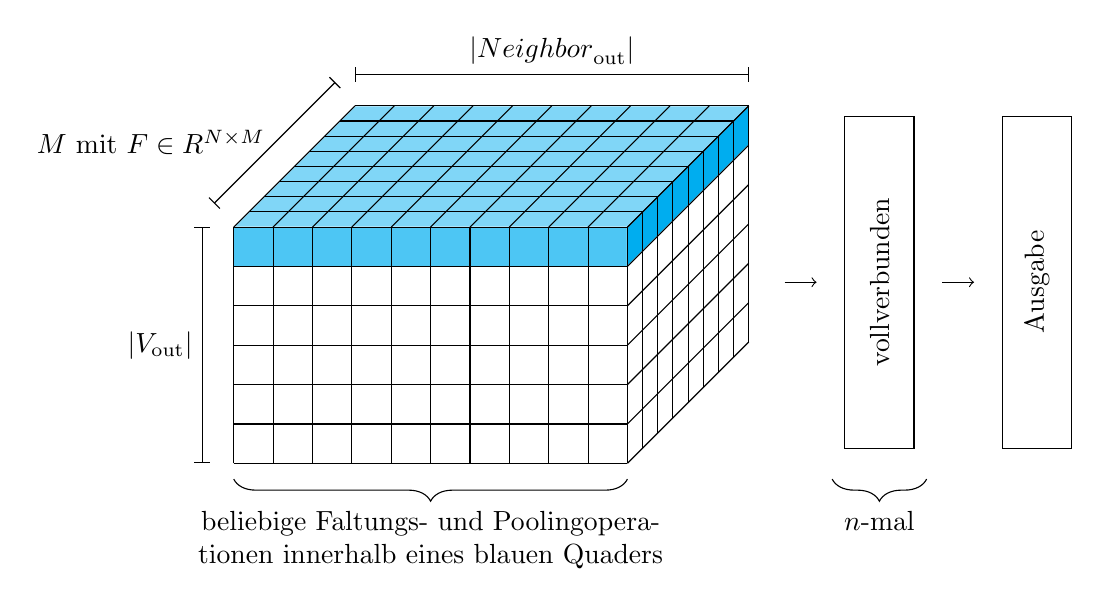
\begin{tikzpicture}
  \draw[white,fill=cyan!70] (0, 3, 4) -- (5, 3, 4) -- (5, 2.5, 4) -- (0, 2.5, 4) -- cycle;
  \draw[white,fill=cyan!50] (0, 3, 4) -- (5, 3, 4) -- (5, 3,   0) -- (0, 3,   0) -- cycle;
  \draw[white,fill=cyan]    (5, 3, 4) -- (5, 3, 0) -- (5, 2.5, 0) -- (5, 2.5, 4) -- cycle;
  \tikzstyle{path}=[->, shorten >= 10pt, shorten <= 10pt]
  \tikzstyle{node}=[rectangle,draw, minimum width=120pt, minimum height=25pt, inner sep=0pt, fill=white, rotate=90]
  \tikzstyle{noborder}=[draw=none,fill=none]

  \foreach \x in {0,0.5,1,1.5,2,2.5,3} {%
    \draw (0,  \x, 4)  -- (5,  \x, 4);
    \draw (5,  \x, 4)  -- (5,  \x, 0);
  }
  \foreach \x in {0,0.5,1,1.5,2,2.5,3,3.5,4,4.5,5} {%
    \draw (\x, 0,  4)  -- (\x, 3,  4);
    \draw (\x, 3,  4)  -- (\x, 3,  0);
  }
  \foreach \x in {0,0.5,1,1.5,2,2.5,3,3.5,4} {%
    \draw (5,  0,  \x) -- (5,  3, \x);
    \draw (0,  3,  \x) -- (5,  3, \x);
  }

  \draw[|-|] (-0.4, 0,    4)    -- node[left]  {$\left|\gls{V}_{\mathrm{out}}\right|$}        (-0.4, 3,    4);
  \draw[|-|] (0,    3.55, 4.65) -- node[left]  {$M$ mit $\ma{F} \in \gls{R}^{N \times M}$}    (0,    3.55, 0.65);
  \draw[|-|] (0,    3.4,  0)    -- node[above] {$\left|\gls{Neighbor}_{\mathrm{out}}\right|$} (5,    3.4,  0);

  \node[node, noborder] (0) at (6.2,  2.3, 4) {};
  \node[node]           (1) at (8.2,  2.3, 4) {vollverbunden};
  \node[node]           (2) at (10.2, 2.3, 4) {Ausgabe};

  \path[path] (0) edge (1);
  \path[path] (1) edge (2);

  \draw [decoration={brace,mirror,amplitude=8pt},decorate,-] (0,-0.2,4) -- node[below=8pt,text width=8cm, align=center] {beliebige Faltungs- und Poolingoperationen innerhalb eines blauen Quaders} (5,-0.2,4);
  \draw [decoration={brace,mirror,amplitude=8pt},decorate,-] (7.6,-0.2,4) -- node[below=8pt] {$n$-mal} (8.8,-0.2,4);

\end{tikzpicture}
\caption[Räumliche Netzarchitektur auf Graphen]{Typische räumliche Netzarchitektur auf Graphen.
Der \emph{Quader}, der durch die Anordnung der Knoten entsprechend ihrer Nachbarschaften entsteht, kann entlang der Nachbarschaften und ihrer Merkmale beliebig oft gefaltet und gepoolt werden.
Eine Faltung entlang der Knotenauswahl besitzt allerdings keine Bedeutung und ist deshalb zu vermeiden.
Im Anschluss können vollverbundene Schichten hin zur Ausgabe an den abgeflachten Quader gestapelt werden.}
\label{fig:netzarchitektur_raeumlich}
\end{figure}


Eigentliche Graphstruktur geht verloren (\zB{} Distanzen der Knoten zueinander) (in gewisser weise stecken diese aber in den Formfeatures).

Die Anordnung der Knoten zu einem Quaderform besitzt damit die Einschränkung, dass das Netz lediglich eine Faltungsschicht enthalten kann.
Die Methode der spektralen Faltung auf Graphen umgeht diese Einschränkung.

Würfel ist speicherineffizient

